%&tex
% !TEX program = xelatex
% !TeX TS-program = xelatex
% !BIB TS-program = biber
% !TeX encoding = UTF-8
% !TeX spellcheck = en_US
% !TeX root = ../thesis.tex
%% ==============================
\chapter{Formal Specification-Based Methods}
\label{sec:formal_methods}
%% ==============================

Two of the most important aspects when programming a~\glspl{acn:plc} are validation and verification.
Validation describes the correctness of the specification compared to the intended use and verification is the correctness of the actual code compared to the specification.
Both of these aspects ensure that the system behaves as intended.
As~\glspl{acn:plc} are used for real-time applications, the importance of these factors increases even more.
The previously described methods for programming with C offered possibilities in that regard, but they did not improve significantly compared to the IEC 61131-3 languages.
Therefore in this section I am investigating the possibilities of using a formal specification to automatically program a PLC.
This allows to easier validate and verify the code that developed.
\citeauthor{Frey:2000aa}\todo{Formal methods in PLC programming} describe different approaches to verification and validation for~\acrshort{acn:plc} programming.
This paper also gives an overview of different methods that can be used to archive this.
From this overview I investigated the three most used techniques in the following section.

There a several methods for creating a formal specification of a process or controller.
One method is to use a formal language to specify the behavior in rules.
This method allows for easier verification and validation as the specification and code can checked via formal theorem solvers.
Approaches employing this method are described in subsection~\ref{sec:sub:flb}.

Another method is to use a modeling language to create a system specification.
A modeling language allows the user to create a structural and behavioral specification of the system.
This is in contrast to the formal languages that only describe behavioral details, but not structures.
They also allow for simulation of the system components making it easier to evaluate and validate the system.
In software development, model specifications like~\acrfull{acn:uml} are common practice.
The usage of a model can also provide a overview of the system and increase modularity.
In subsection~\ref{sec:sub:mb} I investigate approaches using this specification type.

The last approach I investigate are graph based specifications.
They are often used for behavioral descriptions in modeling languages but can also be used just to create a behavioral model.
They use system states and transitions between the states to model a event reaction semantic of the system.
Common approaches here are petri nets and condition graphs.
I describe these approaches in subsection~\ref{sec:sub:graph}.

%% ==============================
\subsection{Formal Language Based}
\label{sec:sub:flb}
%% ==============================

\subsubsection{Linear Temporal Logic}

\acrfull{acn:ltl} is a modal logic that allows to specify conditions over time.
This is done by extending logical operators (and, or, xor, etc.) with temporal operators that specify conditions for the future.
Formally they operate on a sequence of states over the available variables called a Kripke structure\todo{Citation for LTL and Kripke structures.}.
Common temporal operators are~"\textbf{X}~\textit{A}" (Next), specifying that a formula~\textit{A} is true in the next state,~"\textit{A}~\textbf{U}~\textit{B}" (Until), specifying that~\textit{A} is true until~\textit{B} is true and~"\textbf{G}~\textit{A}", specifying~\textit{A} is true in all states.
With these temporal operators a~\acrfull{acn:ltl} formula can specify a full state graph for different variable changes.
A formula is satisfied by a sequence of states~\textit{S} when its true for all states in sequence.
If a formula is~\textit{valid}, it is satisfied for all possible sequences $ S\in 2^{AP} $ given the set of variables~\textit{AP}.

In this section I will investigate two approaches to automated PLC programming that use~\acrshort{acn:ltl} to validate the specification.

\citeauthor{Kuzmin:2013}~\cite{Kuzmin:2013} use~\acrshort{acn:ltl} to specify the behavior of the controller.
They then use the formulas to validate the specification with a model checker and then automatically create a~\acrshort{acn:ST} program.
In this approach, the variables for the~\acrshort{acn:ltl} are all input variables, output variables and state variables that are used in the PLC program.
For specifying the behavior of the controller a~\acrfull{acn:ltl} formula defines the change of a variable given a system condition.
To simplify this process they restrict the values of the variables to boolean and numerical values and only allow one value change per variable per PLC working cycle.
\begin{equation}
GX\left(V > \_V \rightarrow OldValCond \land FiringCond \land V := NewValExpr \right)
\label{eq:increase}
\end{equation}
\begin{equation}
GX\left(V > V \rightarrow OldValCond' \land FiringCond' \land V := NewValExpr' \right)
\label{eq:decrease}
\end{equation}
Equation~\ref{eq:increase} shows the proposed~\acrshort{acn:ltl} formula for increasing a variable V given a~\textit{OldValCond} and a~\textit{FiringCond}, equation~\ref{eq:decrease} show the decrease of V.
They define these conditions for all possible alterations of boolean and numerical values.
The pair of~\acrshort{acn:ltl} for increasing and decreasing a variable can be translated to a ST program block.
\lstset{language=Pascal}
\begin{lstlisting}[caption={
Auto-generated~\gls{acn:ST} code realizing the~\acrshort{acn:ltl} formulas~\ref{eq:decrease} and~\ref{eq:increase}.~\cite{Kuzmin:2013}},label=lst:ltl:st]
IF OldVarCond AND FiringCond THEN
    V := NewValExpr; (*V+*)
ELSIF OldVarCond' AND FiringCond' THEN
    V := NewValExpr'; (*V-*)
END_IF
\end{lstlisting}
Listing~\ref{lst:ltl:st} shows the~\acrshort{acn:ST} code for the equations~\ref{eq:increase} and~\ref{eq:decrease}.
Additionally they propose a transformation to model checker code that allows to verify the integrity of the model.
This is done by finding a sequence of inputs where one of the LTL formula is not satisfied.
If such a sequence is found, it shows that not all LTL formula a valid, which suggests that the specification is incomplete.
If the LTL formulas are valid, there is no possible state of variables where the program is not acting as specified.
With this method, the verification of the control program is easier as it can be done directly from the specification.
But the authors don't provide a formal verification of the transformation and argue with the obvious correctness of the transformation.
This full transformation functions and an example can be found in the paper.

The second approach by~\citeauthor{10.1007/978-3-319-74730-9_23}~\cite{10.1007/978-3-319-74730-9_23} uses a~\acrfull{acn:dsl} to describe the control program.
This~\acrshort{acn:dsl} is then validated by transforming it into~\acrshort{acn:ltl} formula and using a model checker.
The actual~\acrshort{acn:plc} code is created by transforming the~\acrshort{acn:dsl} into a~\acrshort{acn:ST} control program.
They use a event \& response semantic for execution so that the system uses controlled transitions to react to unpredictable environment changes.
The~\acrshort{acn:dsl} allows the engineer to specify a scenario based behavior.
A scenario consists of guarantees, modeling the behavior of the system in a given situation, and assumptions, modeling the assumptions the engineer can make of the environment of the system.
An example from the publication~\cite{10.1007/978-3-319-74730-9_23} for a guarantee would be~"\textit{After picking up an item, the feed arm must move to the press, release the item into the press, and finally move back to the feed belt.}" and one of the related assumptions~"\textit{After a robot arm is instructed to pick up an item, it will eventually pick up that item.}.
These guarantees and assumptions can be specified in the~\acrfull{acn:sml}, the~\acrshort{acn:dsl} they use.
They are defined for every controllable, output entities to define their reaction to input, uncontrollable entities.
Additional keywords for flow control, liveness and safety conditions enable the engineer to give constrains to the specification.
\begin{figure}
	\centering
	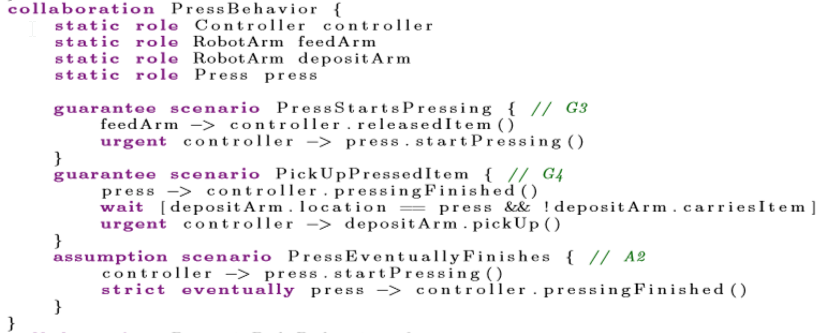
\includegraphics[width=\textwidth]{./Figures/sml_press_beh.png}
	\caption[\acrshort{acn:sml} specification example.]{Example~\acrshort{acn:sml} specification for the behaviour of a press.~\cite{10.1007/978-3-319-74730-9_23}}
	\label{fig:sml_press}
\end{figure}
Figure~\ref{fig:sml_press} shows an example of a behavior formalization.
The wait conditions are for flow control and the urgent statements interrupt the current non urgent operation of the controller and prioritize this task.
They provide a Eclipse based tool named ScenarioTools to create these specifications.
The specification is transformed into a game graph, where nodes are the currently active events and the edges are either controllable or uncontrollable input events.
This graph is a game between the controller and the environment, where the controller tries to reach a state with no liveness scenarios and the environment attempts the opposite.
This can be solved with a General Reactivity of rank 1 solving algorithm.
In this GR(1) problem instance, LTL formula with the form
\begin{equation}
\left(\land_{i}\square\diamond a_{i} \right) \rightarrow \left(\land_{i}\square\diamond g_{i} \right)
\end{equation}
have to be solved, where $a_{i}$ is assumption i is satisfied and $g_{i}$ is guarantee i is satisfied.
If there is a path through the graph where the assumptions hold true but the guarantees do not, its a error in the specification.
This model checking method can be implemented via a~\acrshort{acn:ltl} solver for the transformed GR(1) specification extracted from the~\acrshort{acn:sml} code.
To generate the ST code, this graph is transformed into nested state machines.
Per controller there is a primary state machine modeling the current controller status.
In every possible controller status there are secondary state machines modeling the uncontrollable input components.
The authors state that this transformation is valid by design.

\subsubsection{PLCspecif}

\todo[inline]{PLC Code Generation Based on a Formal Specification Language}

\subsection{Model Based}
\label{sec:sub:mb}

\subsubsection{UML / SysML}

\todo[inline]{Automated PLC Software Testing using adapted UML Sequence Diagrams}

\todo[inline]{A Model-Driven Approach on Object-Oriented PLC Programming for Manufacturing Systems with Regard to Usability}

\todo[inline]{Automatic Generation of Implementation in SysML-based Model-Driven Development for IEC 61131-3 Control Software}

\subsubsection{Simulink}

\todo[inline]{Model-based Verification of PLC programs using Simulink Design}

\todo[inline]{Comparison of a transformed Matlab/Simulink model into the programming language CFC on different IEC 61131-3 PLC environments}


\subsection{Graph Based}
\label{sec:sub:graph}

\todo[inline]{Template-Based Generation of PLC Software from Plant Models Using Graph Representation}

\cite{Frey:2000:2}